\chapter{Pushing the limit of \pangenome construction methods}
\label{sec:pushing}
In this first chapter we present and discuss two situations in which we have pushed the limit of \pangenome constructing methods. In the first one we analyzed the current state of the art methods available at the moment and stress-tested them to generate what was, to the best of our knowledge, the largest human \pangenome produced at the time. The second one was the generation of a yeast \pangenome reference for the species \emph{Lodderomyces elongisporus}. In order to best capture the suspected rearrangement events between 3 chromosomes, we had to modify one of the best known pangenome construction pipeline: this lead to challenges and discussion about how to achieve balance between biological correctness and genome variation resolution of the \pangenome.

\section{Pangenomics and pangenome graphs}
Since the beginning of genomics, all analysis based on sequencing data depended upon the use of a single linear reference genome, i.e. the best assembled genome available for a species, to extract useful information from the DNA. We now know that this approach is suboptimal in a wide range of applications as a lot of genetic material of the species cannot be present in a single linear refererence: this is valid for eukariotes and even more for bacteria.  
This limitation at the beginning was not solvable due to the scarcity of high quality assembled genomes as the technologies of sequencing and computational tools were not mature enough. For example, the Human Genome Project took 13 years to produce its result \cite{humangenomeproject} and the absence of long reads with decent error rate made it impossible to automatically resolve repetitive regions like telomeres and centromeres \cite{human-pangenomics-era}, producing a reference only $92\%$ complete\cite{t2t}. This problem was only solved in 2022 \cite{t2t}. \\
Right now we are witnessing a real revolution in the sequencing. As the price is significantly lowering, also thanks to competition of new companies entering the market, new scientific discoveries and technological advances are leading to a remarkable increase of quality, in term of per-base error rate, and throughput. This means than right now we dispose of a rich wealth of high quality sequencing information to produce hundreds or thousands of new first grade assemblies.
This progress lead to a shift in paradigm with increasing effort from the scientific community to propose new methods to analyse one or multiple genomes: not anymore by comparing it against a single reference sequence but against a comprehensive representation of the species. \\
This novel way to overcome the limits of "linear genomic" and consider all the variation in a single species is called pangenomics. \\
Various efforts are being made on producing reference pangenomes of yeasts, bacterias, plants and animals, including humans. In order to do so, new tools to construct and then analyse and use such representations are being developed. 
It is important here to notice, as it will be stressed in the next sections and chapters, that construction is just the first step and that is very important to understand and work on which are the operations that can be succesfully performed by these representations. 
%The representation more studied and developed at the current moment consists of building a graph that contains the whole genetic material and the variation within a population.

\section{Motivation}
The following paper originates from a discussion early in my PhD journey, on which are the best suited tools for large cohort pangenomes of species with large genomes, like animal or pants. As pointed out in the introduction, there is no one-fits-all solution and  most of the tools, at the time of the analysis, were freshly released or distributed under development. It was therefore \\
In order to evaluate the current state of the art of pangeome builing tools, we decided to perform a thorough assessment of the best available methods by giving as input the largest dataset we could produce to mimic the conditions that they could be required to be used in the near future. We decided to test on human data because of the significance and usefulness of pangenomes of our species. \\
There are multiple ways of representing a group of genomes to be analyzed or used jointly. One that took traction in the last few years has been graphs. Graphs can represent the sequences as labels of nodes, relationship between them (adjacency or overlap) as edges and infer difference in the genomes as different collections of nodes in the graph.
We specifically focused our attention on the most used ones, variation graphs and De Bruijn Graphs, In variation graph edges represent adjacencies, i.e the genome is spelled by a walk on nodes connected by an edge. In De Bruijn Graphs they represent overlaps i.e. the suffix of a node is the prefix of the next node connected to it: this implies that edges can exists between nodes that are not adjecent in the genome. As discussed in the next sessions, this distinction implies several differences in how these graphs can be used for downstream analysis. \\ In this article, we surveyed the the methods and tools that build such graphs, then tested them on different datasets and finally analyzed their features. The result is a small guide on which are the best applications for each of these tools and which are the weaknesses they suffer. \\
The work we performed was intended for publication, but, to the best of my knowledge, the manuscript has never been put in production.

\section{Current limitations: a \emph{Lodderomyces elongisporus} pangenome reference}
Here I present another example of pushing the boundaries of variation graph pangenome building tools, precisely in building graph that represent inter-chromosomal events like rearrangements. This was done when working with the consortium I belong to, the EU Commission founded Marie Curie ITN Alpaca consortium, on builindg a pangenome reference for the medically interesting yeast strain of \lodelo. \\
We sequenced, in collaboration with a lab at the Comenius University in Bratislava, Slovakia, 11 different samples using ONT. The computational work I present here was done in collaboration with members of the consortium, in large part by Simon Heumos, whom I would like to thank for the time spent discussing and working together.
This work was another example of how difficult it is to produce biologically significant pangenome graphs with th current state-of-the-art tools and offers insights on other areas that should be improved. 

\subsection{\emph{Lodderomyces elongisporus}: genetic characteristichs and interest}
\emph{Lodderomyces elongisporus} is a diploid yeast that has been isolated from, among many sources, humans and it is recently emerging as pathogenic. It is phylogenetically placed in the Candida clade and the side of its genome is usually between 15 and 16 Mb, 2 orders of magnitude smaller than a human genome~\cite{Lodderomyces}. Its DNA is organized into 8 chromosomes, named from A to H, of different length from around 3.5Mbp of chr A to 800 Kbp of chr H and a 35 Kbp mitochondrial DNA. Our analysis shows that it has a stable core genome of ~13Mbp.
Increasing reports of (mostly bloodstream) infection in mainly immunosuppressed adults makes it an increasingly important subject of studies: an outbreak war reported occurring in a neonatal ICU in Dheli, India from September 2021 to February 2022 with 1 death\cite{lodelo_india}.
\subsection{Building ad hoc pangenome reference using variation graphs}
Given high quality assemblies generated by the sequencing information we got of these 11 samples, we decided to build a pangenome graph using different tools. As noted in the previous section, \dbgs are very easy and simple to generate, but their usefulness is limited for visual analysis for complex biological events interpretation and study. To this end we also decided to produce variation graphs using first \pggb and then \mcactus, in a similar way to what has been done with the Human Draft Pangenome Reference~\cite{hdpr}, to then inspect the graph and gain knowledge of the kind of variations present between the samples. \\
It is important to notice that in order to produce the best biological correct result, several rounds of parameter tuning and manual curation are needed, with knowledge far superior of the one of a normal user: to this end, Simon help was paramount. Samples were called in alphabetical order from A to K, followed with a number greater or equal than 0 that flagged the version of the assembly. Moreover, one sample, B2, for which a member of the consortium produced a high quality assembly after manual curation, was used as relative reference. Another sample, J, was fully resolved into chromosomes while the others were divided into smaller contigs. \\
\subsubsection{Determining chromosomal communities} 
As variation graphs pangenome construction pipelines use mapping or alignment to infer graphs, the first step consists in grouping together the sequences of all the genomes by chromosome, in order to peform computation separately for any chromosome: each group of sequence will be in processed in a isolated way compared to the one of other groups. The final output graph will have (at least) a separate connected component for every group give as input: this means that without any pre-processing, no inter-chromosomal event can be detected.  
As the rest of the assemblies, with the exception of the J2 sample, were not resolved into single chromosomes, each of them was aligned to the reference B2 using \wfmash alignment segment size of 10k and 95\% sequence identity. The identity scores of the alignment of the genomes to the reference B2 assemby is shown in picture~\ref{fig:lodelo_alignment_scores}.
%Unaligned contigs were aligned with segment size of 100 and 90\% of sequence identity. 
\begin{figure}[t]
	\centering
	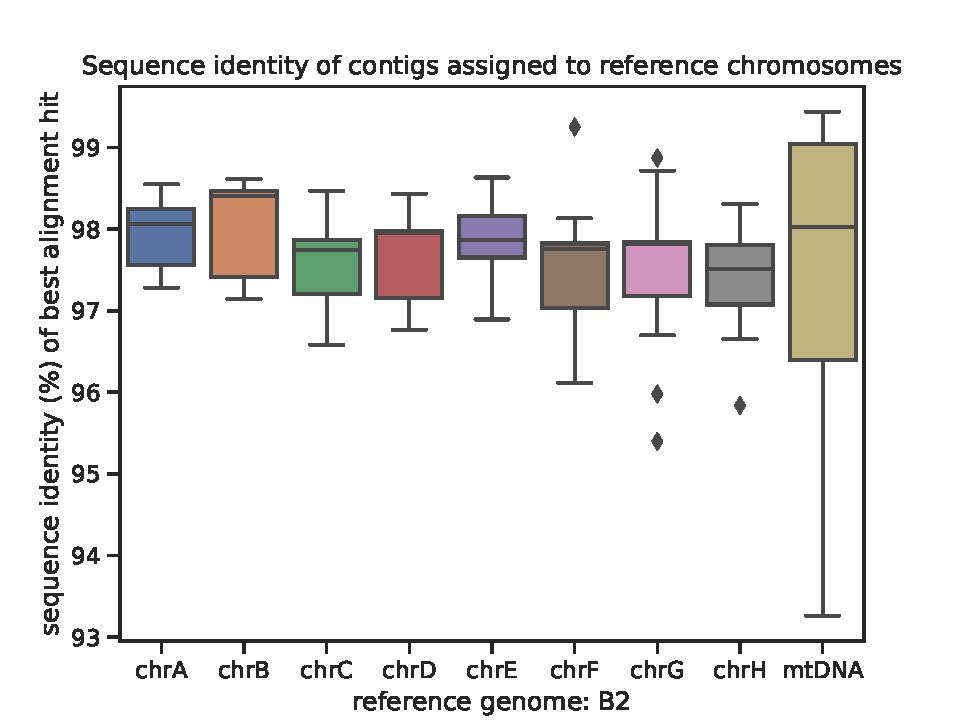
\includegraphics[width=.8\linewidth]{figures/Alignment_scores.pdf}
	\label{fig:lodelo_alignment_scores}
	\caption{Sequence Identity of contigs assigned to reference chromosomes.}
\end{figure}
We detected chromosome-crossing syntenies for multiple contigs in alignment hits of chromosomes C, G, and H, indicating that they correspond to a singular same recombination group: this was consistent with the genomic study, based on SNPs, performed on the isolates related to the Dheli outbreak. In their finding, this is more frequent in hospital/patient populations than in fruit ones~\cite{lodelo_india}. This event was not straightforwardly identifiable from simple community separation, like the one suggested in the manual of \pggb. 
We therefore decided to run the pipelines with just one single community for chromosomes C,G and H.
In figure~\ref{fig:lodelo_communities} it is displayed the community partition of the assemblies based on Louvain algorithm. The latter does not show any condensation of the 3 chromosomes into a single community: this reinforces the fact that "manual" inspection of the alignments is still required in absence of high quality assemblies in order to produce biologically valuable graphs.\\
\begin{figure}[t]
	\centering
	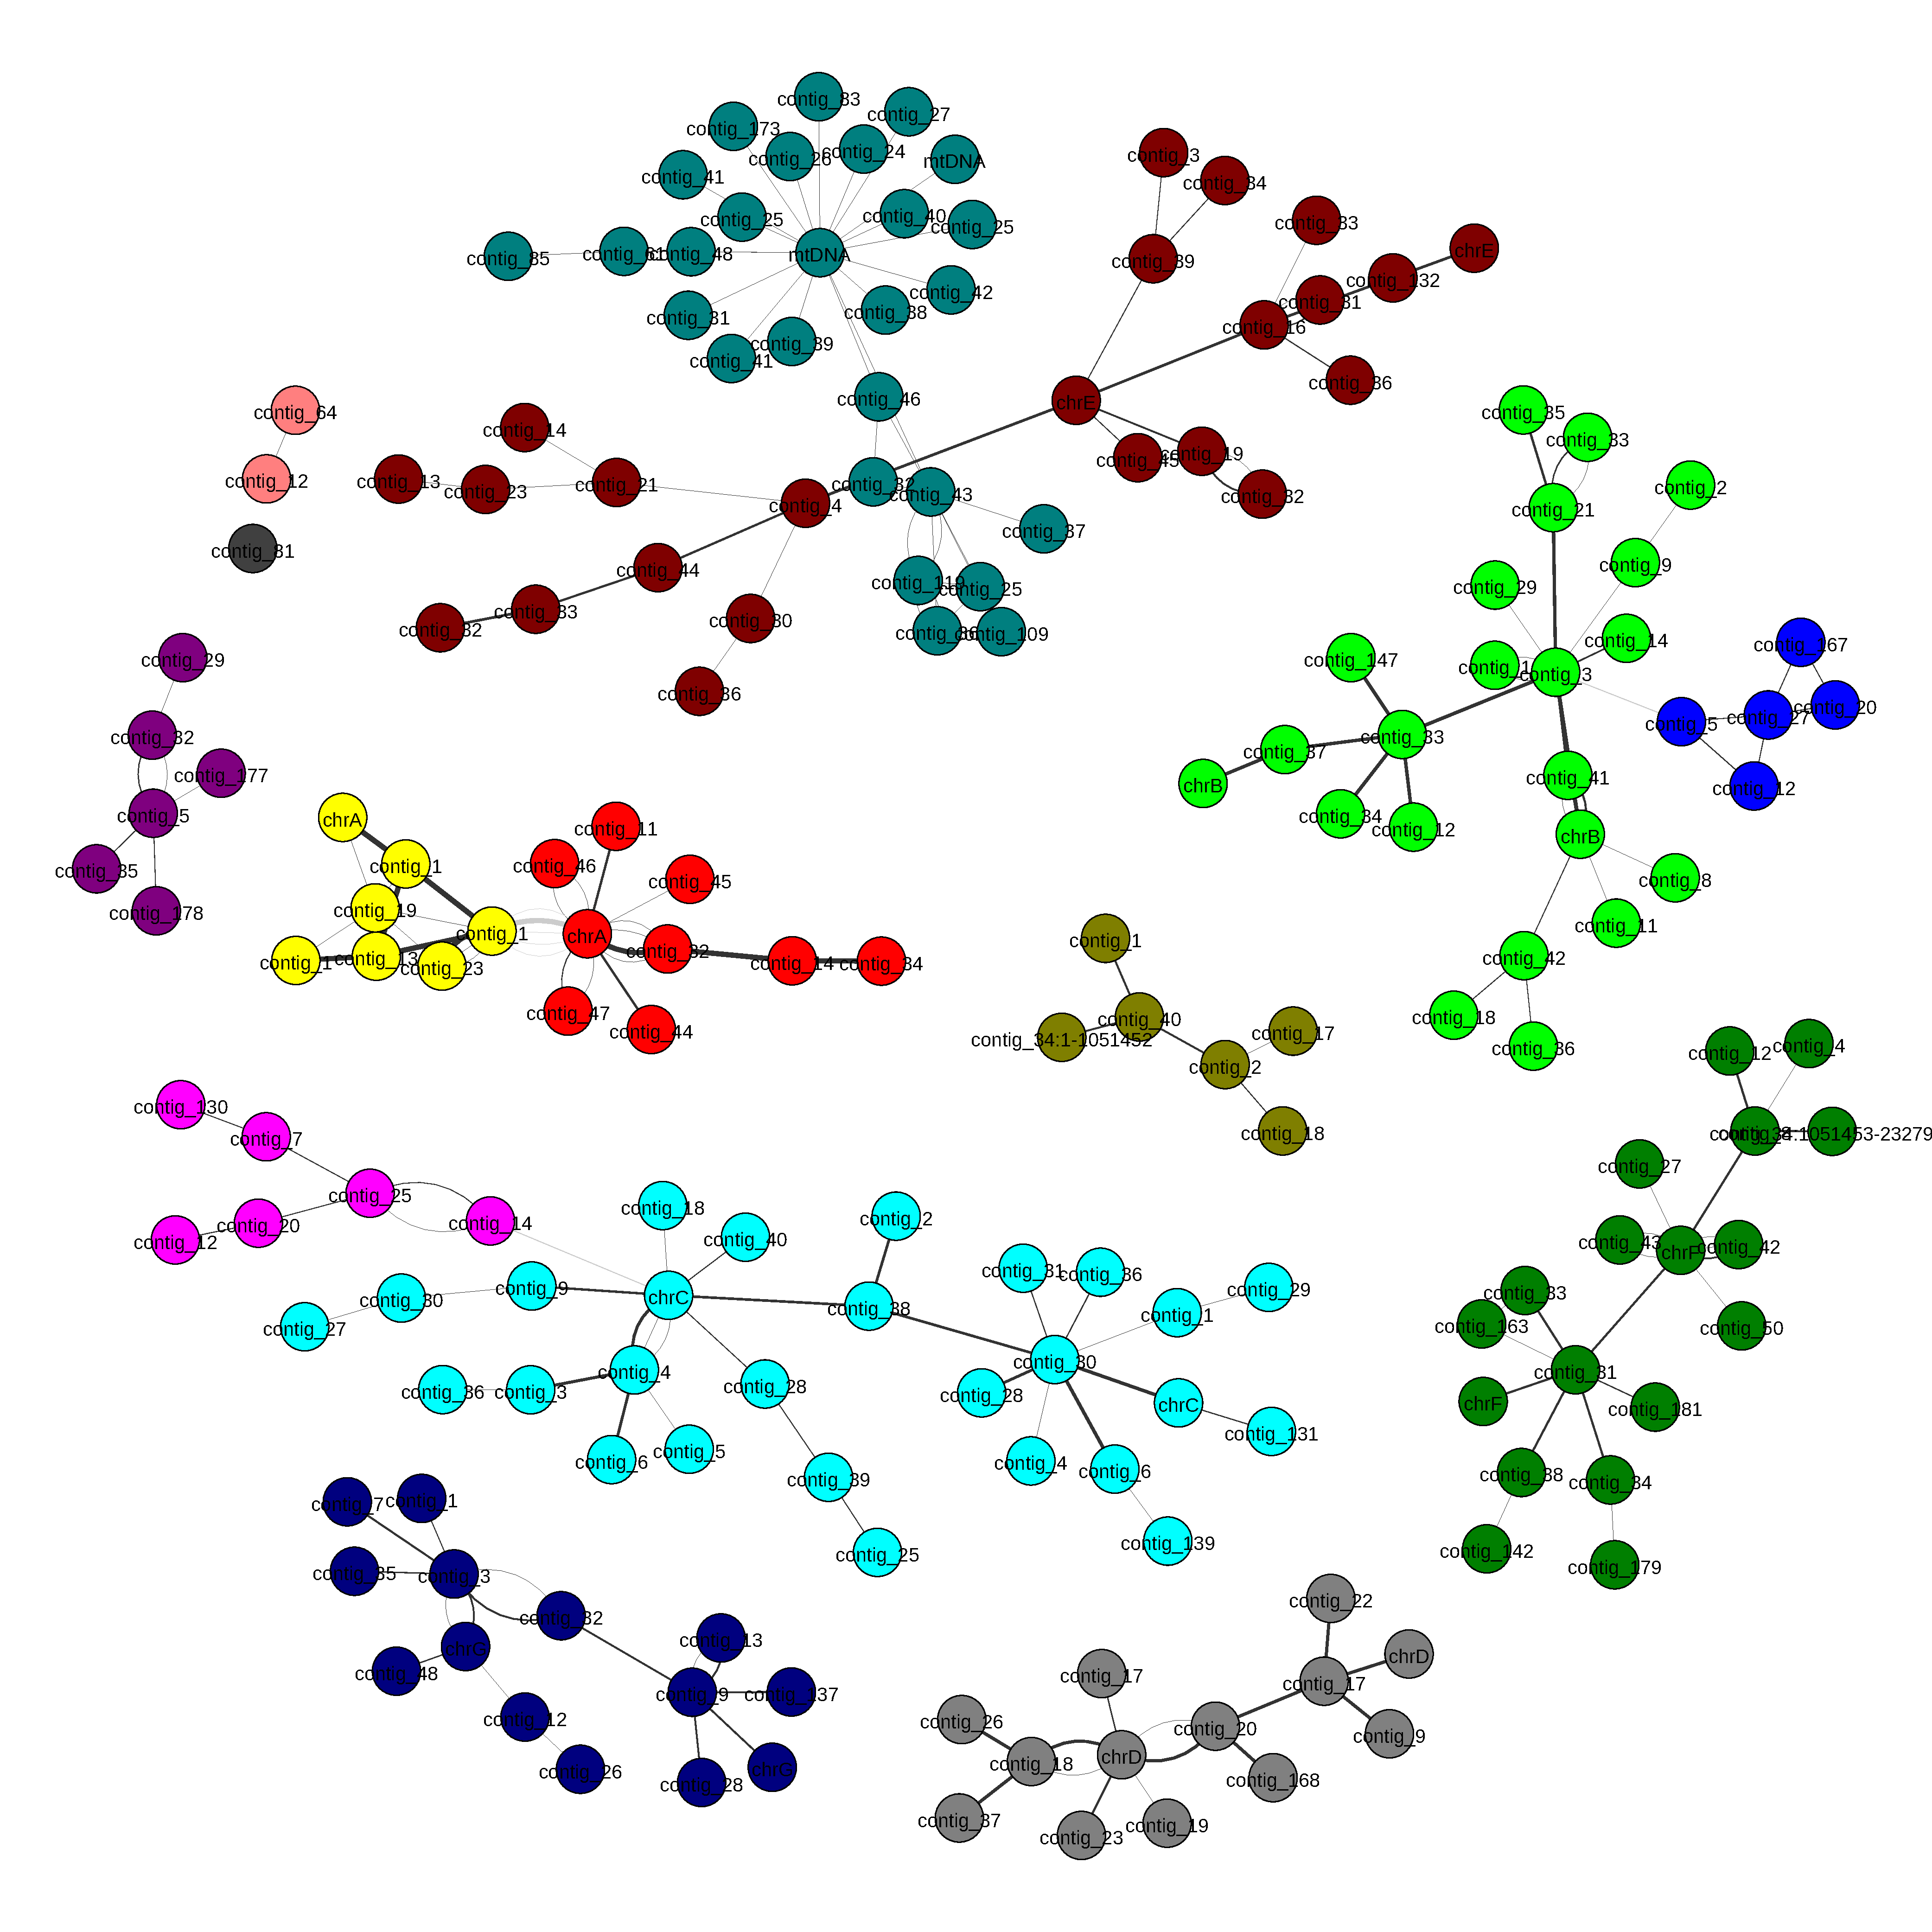
\includegraphics[width=.8\linewidth]{figures/alingment_communities.pdf}
	\label{fig:lodelo_communities}
	\caption{Community partition of the contigs based on alignment scores.}
\end{figure}

\subsubsection{Customizing the pipelines}
As \pggb uses all-vs-all alignment of a collection of sequence as first step to infer the graph, it enables the representation of recombination among chromosomes placed inside the same community, as seen also for human acrocentric chromosomes~\cite{Guarracino2023}.\\
This is not the case for the other well known pipeline for variation graphs construction: \mcactus. As the first step is based on Minigraph, it must have a single reference sequence for any collection of sequence that has to be considered together, be it a single chromosome or a group of them.
This means that there is no feature to have chromosome C,G and H considered together in input. \\
To try to overcome this limitation of the approach we tried to produce a graph that respected the condition of having the three chromosome inside the same connected component of the graph, at the cost of biological correctness. We therefore produced a chimeric contig consisting of the concatenation of the three chromosomes assemblies of the B2 sample. The rationale was to provide it as a backbone so that there is a single reference for the \minigraph construction step. The expectancy was to therefore produce a graph that showed the recombination from the mapping of the contigs of the other genomes. \\
By building a graph using \minigraph with the chimeric chromosome CGH and all the contigs of the other genomes assigned to chromsome C, G and H does not represent any recombination event, as can be seen in figure~\cite{fig:cgh_mingraph}. This was somewhat expected, as it is known that \minigraph does not also consider inversion between genomes.
When the complete modified pipeline of \mcactus is run, it is possible to see the tangle between the chormosomes, as shown in figures~\ref{fig:cgh_mcactus,fig:lodelo_graph_tangle}
\begin{figure}[t]
	\centering
	\begin{subfigure}{\textwidth}
		\centering
		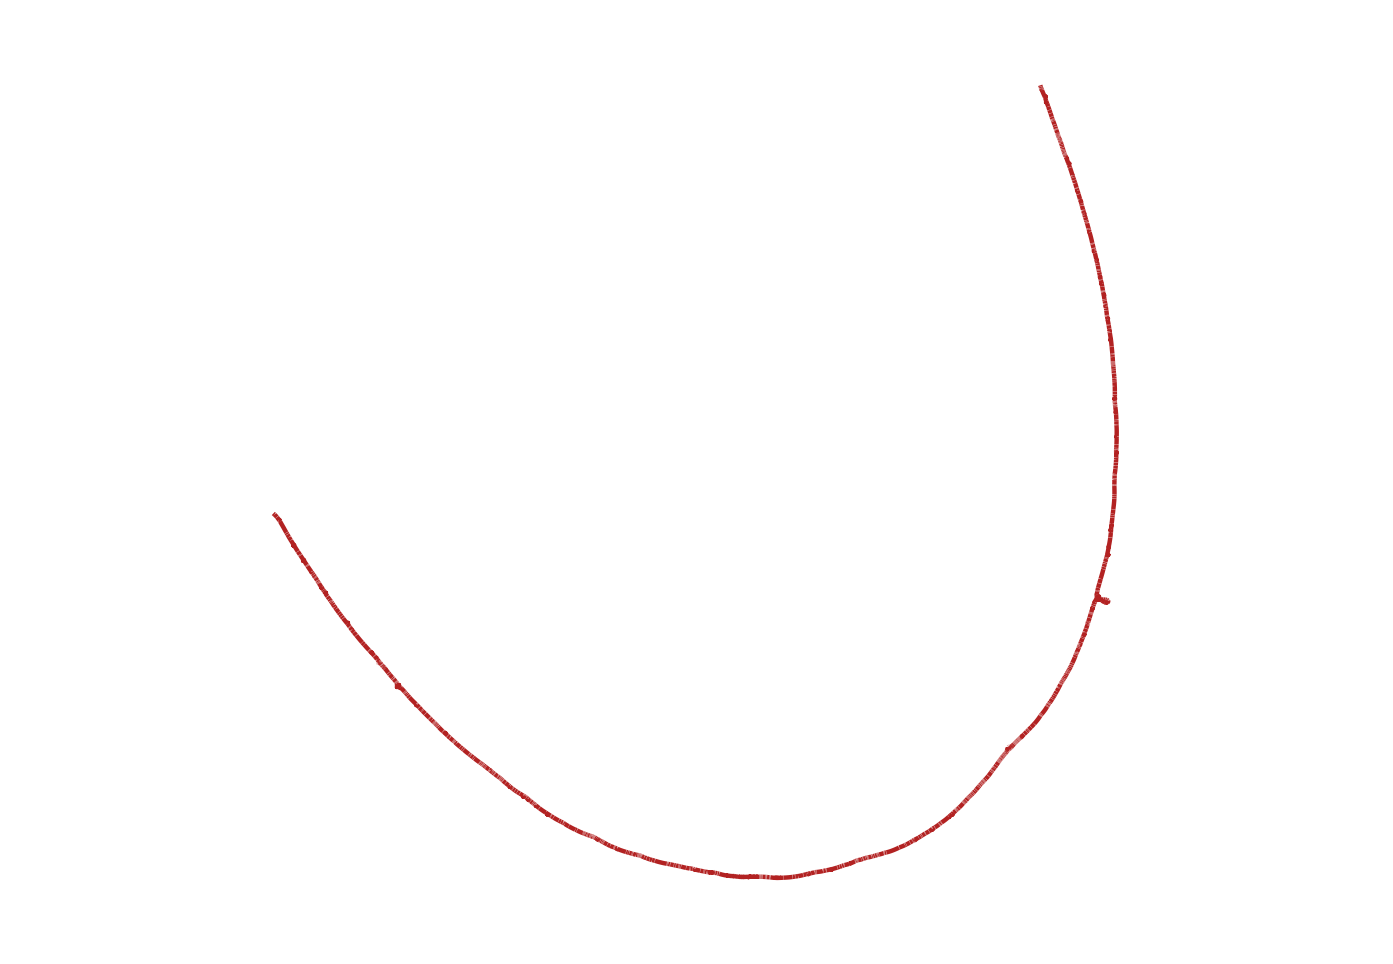
\includegraphics[width=.8\linewidth]{figures/minigraph_cgh.png}
		\caption{Graph of chimeric chromosome CGH from sample B2 and all the contigs of the other genomes aligning to it produced with \minigraph. The graph is linear and no inter-chromosomal event is visible.}
		\label{fig:cgh_mingraph}
	\end{subfigure}%

	\begin{subfigure}{\textwidth}
		\centering
		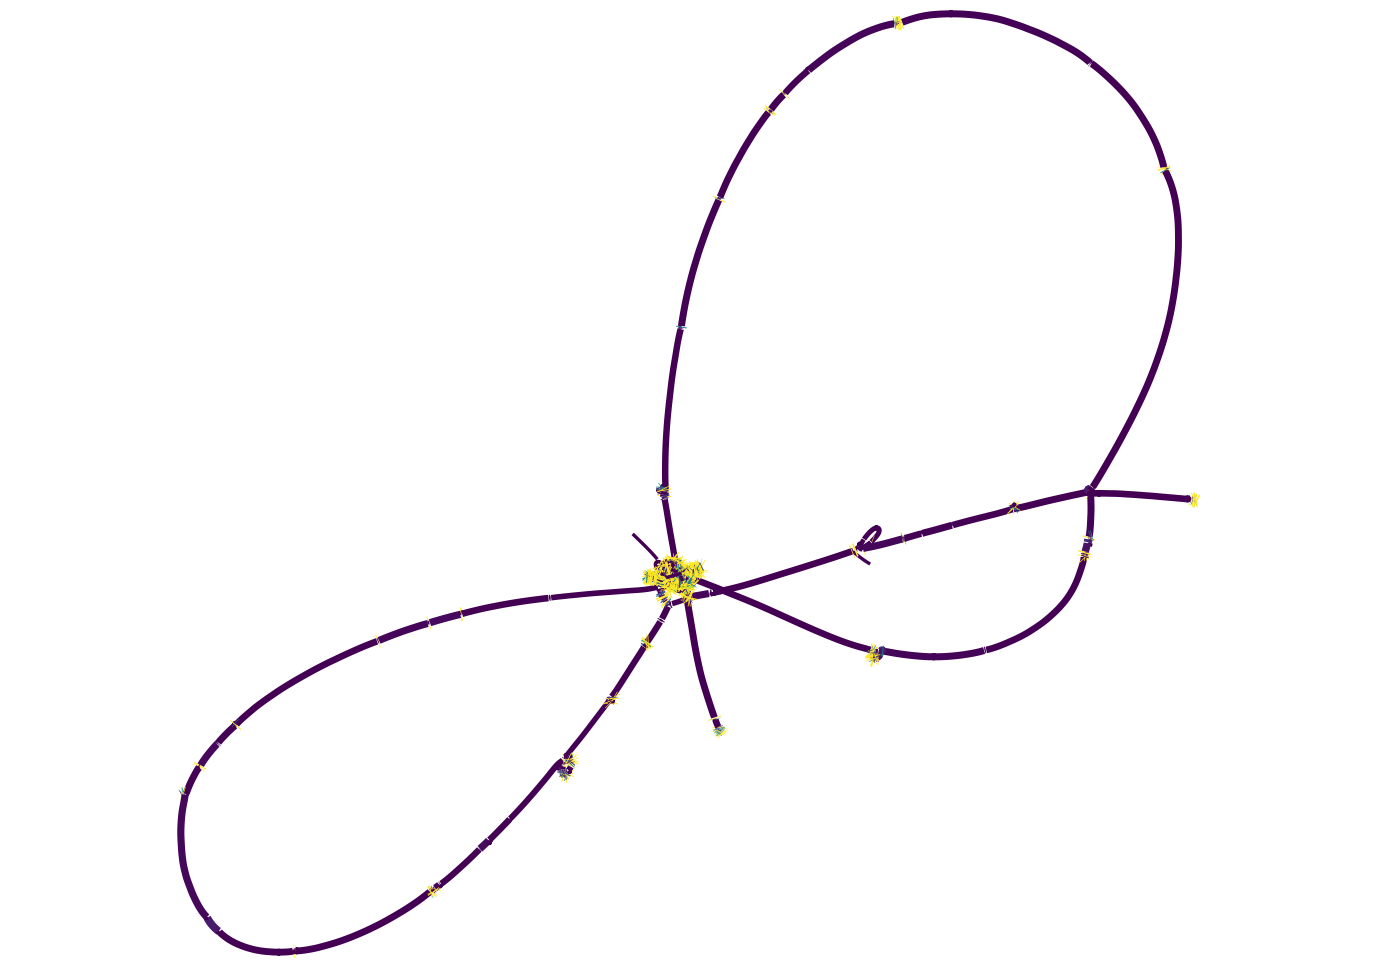
\includegraphics[width=.8\linewidth]{figures/mcactus_cgh_u1000_by_depth.png}
		\caption{The graph after all the other steps of the \mcactus pipeline, coloured by depth, after simplification of variants < 1kbp using the command \gfatools  \texttt{asm -b 1000 -u}. The large recombination event is now visible.}
		\label{fig:cgh_mcactus}
	\end{subfigure}
	\caption{Difference in output between \minigraph and \mcactus of the chimeric graph produced to visualize the inter-chromosomal event between C,G and H.}
	\label{fig:chromosome_cgh_minigraph}
\end{figure}

\subsection{Focus on the tangle}
\begin{figure}[t]
	\centering
	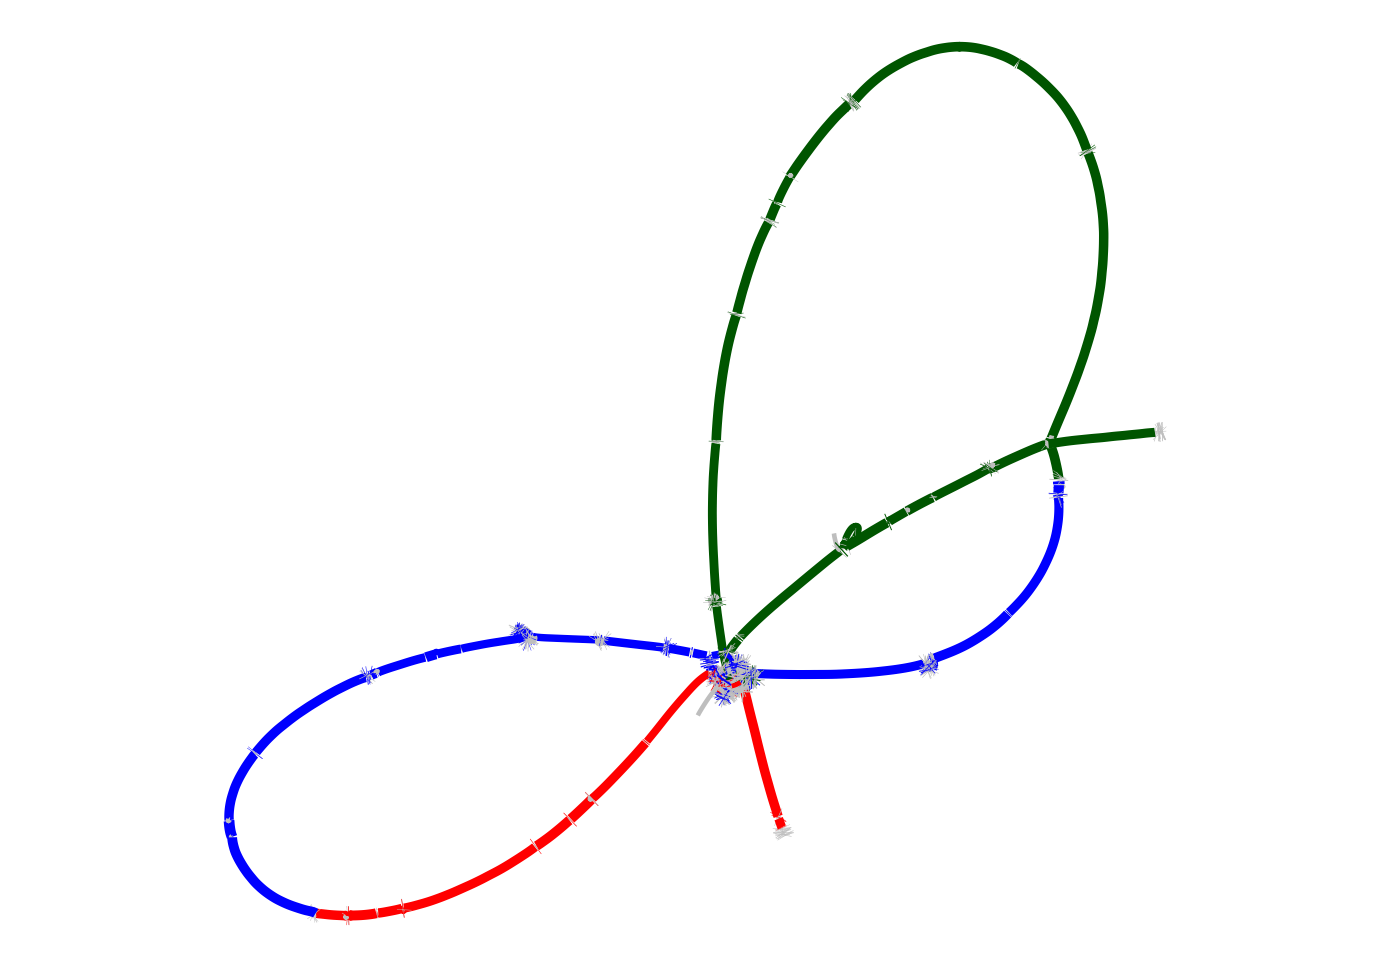
\includegraphics[width=.8\linewidth]{figures/tangle_chrCGH_B2_Cgreen_Gblue_Hred.png}
	\label{fig:lodelo_graph_tangle}
	\caption{The tangle of chromosomes C, G and H in the \mcactus variation graph. Nodes are colored based on \minigraph alignment of chromosome C (dark green), G (blue) and H (red) of the reference assembly B2. The three chromsomes are bound together because of the construction.}
\end{figure}


\section{Conclusion and Perspectives}

\printbibliography